\documentclass[conference]{IEEEtran}
\IEEEoverridecommandlockouts
\usepackage{graphicx}
\usepackage{algorithm}
\usepackage{algorithmicx}
\usepackage{algpseudocode}
\usepackage[dvipsnames]{xcolor}
\usepackage{amsmath}
\usepackage{hyperref}
\usepackage{caption}
\usepackage{subcaption}
\usepackage{ulem}

\algblock{Input}{EndInput}
\algnotext{EndInput}
\algblock{Output}{EndOutput}
\algnotext{EndOutput}
\newcommand{\Desc}[2]{\State \makebox[2em][l]{#1}#2}

\newcommand{\tristan}[1]{\color{orange}\textbf{From Tristan:}#1\color{black}}
\newcommand{\english}[1]{\uwave{#1}}

\newcommand{\valerie}[1]{\color{blue}\textbf{From Valerie:}#1\color{black}}


\begin{document}
\title{I/O simulation model with Linux page cache, integration and evaluation in SimGrid framework}

\author{\IEEEauthorblockN{Hoang-Dung Do$^1$, Val\'erie Hayot-Sasson$^1$, Rafael Ferreira da Silva$^3$, Henri Casanova$^2$, Tristan Glatard$^1$
  }\\
  \IEEEauthorblockA{
    $^1$Department of Computer Science and Software Engineering, Concordia University, Montreal, Canada\\
     $^2$Department of Information and Computer Sciences, University of Hawai‘i at Manoa, USA\\
     $^3$Department of Computer Science, University of Southern California, Los Angeles, USA
  }
}

\maketitle

    \begin{abstract}
        
        The rapid emergence of Big Data seen in recent years has resulted in a 
        growing needs for efficient data storing and optimized data analysis. 
        Despite relying on large computing infrastructures with powerful computing capability 
        to process these large datasets, an I/O bottleneck remains. 
        One widely-used approach to minimize the costs of data transfers during
        regular use is through the employment of the page cache.
        While many simulation tools have been developed to 
        support studies in computing systems optimization, page cache simulation 
        has not been fully captured or remains absent from these simulators. 
        The lack of ability to simulate I/O with page cache leads to inaccurate 
        simulation results in many situations, especially when dealing with data intensive applications. 
        
        In this paper, we propose a I/O simulation model that characterizes the key features of the page cache.
        We have implemented the model with SimGrid, a simulation framework for 
        distributed systems, using WRENCH, a SimGrid-based workflow simulator. 
        Our simulator is compatible with both single-threaded and multithreaded applications,
        and can simulate both writeback and writethrough cache that can factor into local
        and network-based filesystems.
        The results show that our simulator not only achieves higher accuracy than 
        original WRENCH, but also effectively simulates memory contents and 
        page cache during I/O operations. 
        Through this study, our effort is to contribute an analytical model 
        of the page cache, which can also be integrated to other simulators 
        to improve I/O simulation accuracy, with its practical results. 
        
    \end{abstract}         

    \section{Introduction}
        
        In recent years, as a result of the growing demand for Big Data processing 
        on large computing infrastructures, there have been the research and development 
        of simulation applications and frameworks for distributed systems. 
        These simulation tools have shown their advantages in evaluation 
        of algorithms, applications and solutions. 
        Experimenting on real platforms exposes shortcomings due to limited and 
        shared resources, operational costs, unstable environments and the result 
        reproducibility difficulties.
        On the contrary, simulators provide to researchers the freedom of choosing 
        simulated infrastructures, reproducible results and low costs.
        These simulators are developed and integrated with simulation models 
        of computing resources including CPU, network and storage.
        The ultimate goal that all simulators try to achieve is to accurately simulate 
        applications. 
        However, there is a trade-off between accuracy and scalability, which has been 
        indicated in some reviews \cite{casanova2014simgrid} \cite{byrne2017review}. 
        This means that in most ciscumstances, users have to, more or less, sacrifice 
        accuracy for the scalability and performance when their platforms grow to 
        hundreds or thousands nodes. 
        
        Beside computing resources such as CPU, network, storage, another 
        important factor that has significant impacts on I/O performance is 
        page cache. 
        Page cache is an architectural solution employed in systems to tackle 
        the problem of disk I/O bottleneck in data processing. 
        Although this is not a radical solution for disk performance, it contributes 
        to minimizing disk accesses and maximizing I/O performance. 
        Surprisingly, page cache has not been fully modeled, if not completely absent, 
        in simulation tools. 
        Some simulators try to simulate I/O with page cache, but fail to capture the 
        key features such as dirty data and cache eviction mechanism 
        \cite{nunez2012simcan} \cite{nunez2012icancloud}.
        Again, these simulators also have a problem in scalability with 
        long simulation time regarding to their very detailed level of simulation. 
        Other works are able to capture important features of page cache, 
        but they focus on very specific domains, such as energy consumption 
        in \cite{xu2018saving}.

        In this work, we propose a simulation model of I/O with page cache, 
        implement it with SimGrid, a simulation framework for distributed computing, 
        and WRENCH, an open-source library for developing workflow simulator 
        built on top of SimGrid. 
        One of the reasons for us to choose SimGrid is that it has a balance 
        between accuracy and scalability. Moreover, the versatility of SimGrid 
        enables it to be used in cross-domain \cite{casanova2014simgrid}. 
        In addition, SimGrid has been actively maintained with updated documents. 
        Then we evaluate our model with four simulators in four experiment scenarios. 
        This paper is organized as follows. 
        In Section \ref{relatedwork} we provide details of page cache 
        existing simulation tools.
        In Section \ref{relatedwork} we propose our I/O with page 
        cache simulation model and how we implement it and our experiments 
        to evaluate the model.  
        Section \ref{results} compares the results of our model with the results 
        of original WRENCH and real execution results. 
        Finally, Section \ref{discussion} concludes and presents future 
        work.  
        
    \section{Related Work}        
    \label{relatedwork}    
        
        \subsection{Page cache}                            
            
            Linux implements a disk cache called \textit{page cache}. 
            It contains pages referring to physical pages on disk \cite{linuxdev3rd2010}.
            The goal of the page cache is to avoid disk I/O by keeping data in memory 
            for later accesses, minimize I/O time since disk accesses are considerably 
            slower than memory accesses.
            When the kernel starts a read operation, it checks if required data is in page cache.
            If yes, data is read from memory. This is called a \textit{cache hit}. 
            Otherwise, data is read from disk and placed in page cache.
            For writing, page cache is implemented with three different strategies. 
            The first is \textit{direct~I/O} or \textit{no-write}, which means the page cache 
            is not involved in write operations. 
            The second is \textit{write-through}, in which data goes \textit{through} 
            page cache to disk. In this case, data is written to both page cache and disk. 
            In the third strategy, called \textit{writeback}, data are written directly 
            to disk as \textit{dirty} pages and these pages will be periodically flushed 
            to disk later by a \textit{writeback} process and then marked as not dirty. 
            The writeback strategy is considered to outperform write-through as well as 
            direct I/O as it delays disk writes and perform a bulk write later.
            \cite{linuxdev3rd2010}. 
            
            In writeback, one of the keys is the cache eviction mechanism, which is
            triggered when available memory is insufficient to removes pages 
            from page cache. 
            Because dirty pages are data written to page cache but yet to be 
            written to disk, dirty pages must be kept in page cache and only clean pages 
            are available for eviction.
            If the clean pages are inadequate, dirty pages are flushed to disk, 
            marked as clean and available for eviction. 
            There is another type of flushing mechanism, which is 
            \textit{periodical flushing}, called periodically in predefined intervals. 
            Periodical flushing only flushes expired dirty pages, which remain dirty in 
            page cache longer than an expiration time configured in the kernel. 
            Different cache eviction algorithms have also been developed and proposed
            \cite{owda2014comparison}.
            In Linux kernel, a \textit{two lists strategy (LRU/2)} is implemented based on 
            the least-recently-used (LRU) scheme, with an \textit{active list} and 
            an \textit{inactive list}. 
            If accessed pages are not in the page cache, they are added to the inactive list. 
            If pages are accessed when residing in the inactive list, they will be moved from 
            inactive list to active list. 
            The lists are also kept balanced by moving pages from the active list
            to the inactive list when the active list grows too large.
            Thus, the active list only contains pages which are accessed more than once 
            and not evictable, while the inactive list includes pages accessed once only, 
            or pages accessed more than once but moved from the active list. 
            The lists work in LRU manner, pages are added to the tail and removed 
            from the top. 
             
        \subsection{Simulators}
            
            Many simulation frameworks and applications have been developed 
            in recent years to support studies in grids, cloud, HPC, peer-to-peer 
            networks, volunteer computers.                     
            These simulators are built with models of resources such as CPU, network, 
            storage with different approaches and levels of details in different simulators. 
            The detail level of the model causes a conflict between accuracy and scalability, 
            and these simulators usually trade of one for the other 
            \cite{casanova2014simgrid}. 
            For example, some simulators are built with packet-level network models 
            such as \textit{CloudSim} and \textit{iCanCloud}, or storage model that 
            simulates the operation of storage hardware in \textit{DiskSim} 
            \cite{casanova2014simgrid}. 
            Fine-grained models allow simulators to achieve high accuracy, 
            but at the same time lead to scalability issues due to long simulation time 
            when simulated platforms and applications grow. 
            SimGrid is an open source simulation platform that has been developed 
            not only to balance the trade-off between accuracy and scalability, 
            but also to achieve versatility, which allows the use of the framework 
            to simulate applications in multiple domains \cite{casanova2014simgrid}.
            
            Despite the fact that many sophisticated models for resources have been 
            integrated in simulators, and the page cache shows apparent impacts on I/O
            performance, the simulation model of page cache is still missing in most 
            of simulators.
            For example, SimGrid only simulates I/O operations with storage bandwidths 
            and capacity. 
            SIMCAN is a simulation framework that models page cache by storing data 
            accessed on disk in a block cache \cite{nunez2012simcan}. 
            Page cache is also modeled in iCanCloud simulator with a component in charge 
            of managing memory accesses and cached data \cite{nunez2012icancloud}, 
            but one of the issues is scalability due to its sophisticated model.
            Ultimately, non of these simulators provide any cache write strategy, 
            cache eviction mechanism with dirty/clean data and the page cache LRU lists. 
            Cache replacement policies is applied in \cite{xu2018saving} to simulate 
            in-memory caching, but for the study in energy consumption of multi-tier 
            heterogenous network.
            
            In this study, we chose SimGrid to implement our model of I/O with page cache 
            due to the balancing between accuracy and scalibility, the versatility allowing it 
            to be adopted in different domains. 
            In addition, it is an actively maintained open-scource framework with 
            modular design, which enables the framework to be extended with new models. 
            The main issue users have to face when using SimGrid is everything has to be 
            implemented from scratch due to its low-level API. 
            To ease this challenge, WRENCH, another open-source library, is built on top 
            of SimGrid to abstract the low-level logic and expose a higher abstraction 
            level API \cite{casanova2018wrench}. 
            We integrate our model in WRENCH and use the SimGrid API to interact with 
            simulated storage resource.
            This approach allows us to leverage existing features in WRENCH and SimGrid.
            Firstly, we can take advantage of the process control, synchronization of 
            resource consumption by concurrent processes provided by the simulation core 
            in SimGrid. 
            Secondly, we can reuse the existing SimGrid storage model with capacity 
            and bandwidth properties, which are similar to the characteristics of memory.
            And finally, WRENCH provides a high level abstraction, which help us drop 
            the burden of implementation. 
            
    \section{Method}
    \label{method}
    In this section, we present our page cache simulation model for file I/O,
    flusing, and eviction. We detail the design and implementation of two simulators:
    (1) a standalone Python prototype to evaluate the simulation model independently of any other 
    tool, and (2) WRENCH-cache, an extension of WRENCH with our page cache model.
    We also describe experimental scenarios to evaluate our simulators in various configurations.
     
    We separate our simulation model in two components, the IO
    Controller and the Memory Manager, which together simulate 
    file reads and writes in Linux (Figure~\ref{fig:interaction}). 
    To read or write a file chunk, a simulated application sends a
    request to the IOController. The IOController interacts as needed with
    the Memory Manager to free memory through flushing or eviction,
    and to read or write to cache. The Memory Manager
    implements these operations, simulates periodical flushing
    and eviction from cache, and reads or writes to disk when necessary.
    \begin{figure}
           \centering
           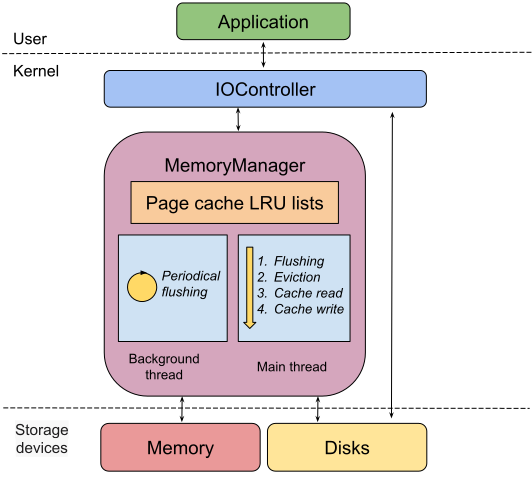
\includegraphics[width=0.85\columnwidth]{figures/interaction.pdf}
           \caption{Overview of the simulated writeback page cache.
           Applications send file read or write requests to the
           IOController that orchestrates flushing, eviction, cache
           and disk accesses with the MemoryManager. Storage
           devices (memory and disk) simulate file transfers with
           bandwidth sharing. \tristan{Could you annotate arrows to
           make them more explicit?}.}
           \label{fig:interaction}
    \end{figure}

    \subsection{Memory Manager}

    The Memory Manager simulates two parallel threads: the main one
    implements flushing, eviction, and cache I/Os synchronously, whereas
    the second one, operating in the background, periodically searches for
    expired dirty data in page cache LRU lists and flushes them to disk. We
    use existing storage simulation models~\cite{lebre2015} to simulate
    memory, characterized by its storage capacity, read and write
    bandwidths, and latency. Reusing existing storage models allows us to
    simulate bandwidth sharing between concurrent memory accesses.

    \subsubsection{Page cache LRU lists}

    In the Linux kernel, page cache LRU lists contain file pages. However, 
    due to the large number of file pages, managing lists of pages 
    induces substantial overheads.
    Therefore, we introduce the concept of a data block as a unit to represent data 
    cached in memory. A data block is a subset of file pages stored in
    page cache that were accessed in the same I/O operation. 
    A data block has information about file name, block size, last access 
    time, a dirty flag that represents whether the data is clean (0) 
    or dirty (1), and an entry (creation) time.
    Blocks can have different sizes and a given file can have multiple 
    data blocks in page cache. In addition, a data block can be split into an 
    arbitrary number of smaller blocks.
    \begin{figure}
           \centering
           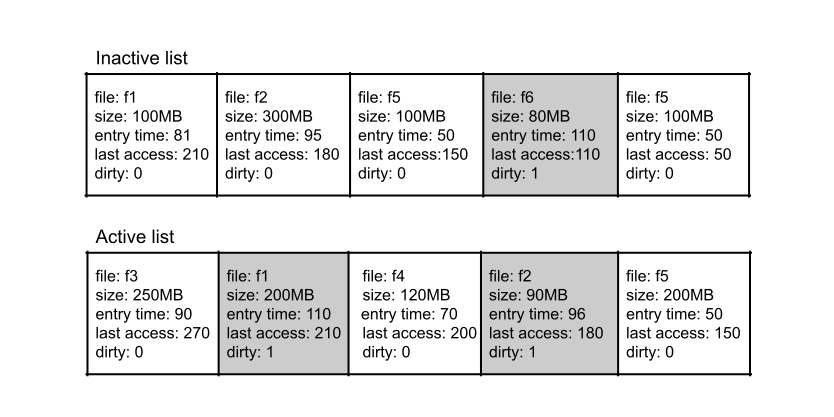
\includegraphics[width=\columnwidth]{figures/lru_lists.pdf}
           \caption{Model of page cache LRU lists with data blocks.}    \label{fig:lrulist}
    \end{figure}    
    
    We model page cache LRU lists as 
    two lists of data blocks, an active list and an inactive list, both ordered by 
    last access time (earliest first, Figure~\ref{fig:lrulist}).
    As in the kernel, our simulator limits the size of the active list to
    twice the size of the inactive list, by moving least recently 
    used data blocks from the active list to the inactive list~\cite{gorman2004understanding, linuxdev3rd2010}.
    % Modeling page cache LRU lists as lists of data blocks reduces the
    % overhead of the simulator, as data blocks are obviously less
    % numerous than file pages. At the same time, it achieves the accuracy in 
    % I/O time simulation that can be seen in the later section.
    % From Tristan: I don't think the sentences above are necessary,
    % they are quite repetitive.

    At any given time, a file can be partially cached, completely cached,
    or uncached at all. Cached data blocks may reside in one or both of the
    page cache LRU lists. The first time they are accessed, blocks are
    added to the inactive list. On subsequent accesses, blocks of the
    inactive list are moved to \tristan{if they are moved then they can't
    be in both lists} the top of the active list. Cached blocks written to
    cache are marked as dirty until they are flushed to disk.

    \subsubsection{Reads and Writes}

    Our simulation model supports chunk-by-chunk file accesses
    with a user-defined chunk size. However, for simplicity, we assume that file pages are 
    accessed in a round-robin fashion rather than fully randomly. 
    Therefore, when a file is read, cached data is read only after all uncached data was read, and data from the inactive list is read
    before data from the active list
    (left to right in Figure~\ref{fig:read_order}).
    When a chunk of \emph{uncached} data is read, a new clean block is created 
    and put at the top of the inactive list. 
    When a chunk of \emph{cached} data is read, one or more existing data blocks in the LRU lists are accessed.
    If these blocks are clean, we merge them together, update the access time and size of the resulting block, 
    and put it in the active list. 
    If the blocks are dirty, we move them to the active list to preserve their entry time. 
    Because the chunk size and block size can be different, there are situations
    where a block is not entirely read. 
    In this case, the block is split in two smaller blocks and one of them is re-accessed.
    % From Tristan: not sure where to put this nor if it's necessary:
    % , in which chunks are read/written
    % until file is entirely read/written.
    \begin{figure}
           \centering
           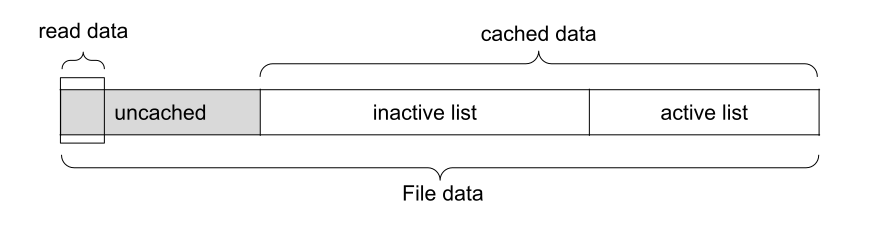
\includegraphics[width=\columnwidth]{figures/read_order.pdf}
           \caption{File data read order. Data is read from left to right: uncached data 
           is read first, followed by data from the inactive list, and finally data from the active list.}
           \label{fig:read_order}
    \end{figure}    

    For file writes, we assume that all data to be written is 
    uncached. Thus, each time a chunk is written, we create a block of dirty data 
    and add it to the inactive list.

    \subsubsection{Flushing and eviction}

    \paragraph*{Flushing}
    The main simulated thread in the Memory Manager can flush the
    cache to write dirty data to disk. The data flushing simulation
    function takes the amount of data to flush as parameter. While
    the amount of data to flush is not reached and there are dirty
    blocks remaining in cache, this function traverses the sorted
    inactive list, then the sorted active list, and writes the
    least recently used dirty block to disk having set its dirty
    flag to 0. In case the amount of data to flush requires that a
    block be partially flushed, the block is split in two blocks,
    one that is flushed and one that remains dirty. Flushing time
    to disk is simulated with the storage model.
    
    \paragraph*{Cache eviction}
    Similarly to data flushing, our cache eviction simulation runs in
    the main thread. It frees up the page cache by traversing and deleting 
    least recently used clean data blocks in the inactive list.
    The amount of data to evict is passed as a parameter and data blocks are deleted 
    from the inactive list until total evicted data reaches the required amount,
    or until there is no clean block left in the list.
    If the last evicted block does not have to be entirely evicted, the block is split in two blocks,
    and only one of them is evicted.
    The cache eviction simulation does not contribute to the simulated time 
    since cache eviction time is negligible in real systems \tristan{a reference would be welcome}.
    
    \begin{algorithm}\caption{Periodical flushing simulation}\label{alg:pdflush}
        \small
        \begin{algorithmic}[1]
            \Input
                \Desc{in}{page cache inactive list}
                \Desc{ac}{page cache active list}
                \Desc{t}{predefined flushing time interval}
                \Desc{exp}{predefined expiration time}
                \Desc{sm}{storage simulation model}
               \EndInput
               \While{host is on}
                \State blocks = expired\_blocks(exp, in) + expired\_blocks(exp, ac) 
                \State flushing\_time = sm.write(blocks)
                \State flag blocks as clean data \tristan{a bit informal}
                \If{flushing\_time $<$ t}
                    \State sleep(t - flushing\_time)
                \EndIf \tristan{else?}
            \EndWhile
        \end{algorithmic}
    \end{algorithm}

    \paragraph*{Periodical flushing}
    Periodical flushing is simulated in the Memory Manager
    background thread. As in the Linux kernel, a dirty block
    in our model is considered expired if (1) it is dirty, and (2)
    the duration since its entry time is longer than a
    predefined expiration time. 
    Periodical flushing is simulated as an infinite loop in which 
    the Memory Manager searches and flushes these expired dirty blocks to disk (Algorithm~\ref{alg:pdflush}). 
    % From Tristan: the algorithm is quite straightforward, I don't think this is 
    % necessary
    % In each repetition, Memory Manager finds expired dirty blocks in two 
    % page cache LRU lists (line 8), simulates writes of data of these blocks 
    % to disk (line 9), and mark them as clean (line 10).
    % If the flushing time does not exceed our time interval, the thread is put 
    % to sleep for the remaining time (lines 11-13). 
    % Then based on the state of the host at current simulated time, 
    % the algorithm continues or finishes the loop.
    Because periodical flushing is simulated as a background thread, it can happen concurrently
    with disk I/O initiated by the main thread. This parallelism is handled by the 
    storage model and reflected in simulated I/O time.

    \subsection{I/O Controller}
     
    \begin{algorithm}\caption{File chunk read simulation of IOController}
    \label{alg:read}
        \small
        \begin{algorithmic}[1]
            \Input
                \Desc{cs}{chunk size}
                \Desc{fn}{file name}
                \Desc{fs}{file size (assume to fit in memory)}
                \Desc{mm}{MemoryManager object}
                \Desc{sm}{storage simulation model}
               \EndInput
               \State disk\_read = min(cs, fs - mm.cached(fn))
               \State cache\_read = cs - disk\_read
            \State mm.flush(cs + disk\_read - mm.free\_mem - mm.evictable, fn) 
            \State mm.evict(cs + disk\_read - mm.free\_mem, fn) 
            \If {disk\_read $>$ 0}  \Comment{Read uncached data}    
                \State sm.read(disk\_read)  
                \State mm.add\_to\_cache(disk\_read, fn)     
            \EndIf
            \If {cache\_read $>$ 0} \Comment{Read cached}
                \State mm.cache\_read(cache\_read)  
            \EndIf
        \end{algorithmic}
    \end{algorithm}            
    As mentioned previously, our model reads and writes file chunks in a round-robin 
    fashion.
    When a simulated application reads a file chunk, it sends a chunk read request 
    to IOController.             
    The algorithm to simulate a chunk read implemented in IOController 
    is described in Algorithm~\ref{alg:read}.   
    First, we calculate the amount of uncached data that needs to be read 
    from disk, and the remaining amount is read from cache (line 7-8).
    We assume that after a file is read, there are two copies of the file in memory 
    (one in cache, one in anonymous memory). 
    Unfortunately, SimGrid lacks of application memory management and WRENCH 
    only use the memory capacity to check if the applications can be run. 
    Thus, in our model, when a chunk is read, one copy of the chunk 
    occupies anonymous memory, and the uncached part of that chunk is 
    read into cache.    
    The amount of required memory to read the chunk is calculated and 
    if there is not enough memory available, Memory Manager is called to 
    flush dirty data to disk and simulate flushing time with memory model (line 9). 
    This flushing is complemented by eviction in the Memory Manager (line 10). 
    Then, if there is uncached data, a disk read is simulated with disk model (line 12), 
    and this data of the file is added to cache (line 13).
    Finally, if cached data is read, Memory Manager is called to simulate a cache read  
    and update the corresponding data blocks in cache (line 16).
    \begin{algorithm}\caption{File chunk write simulation of IOController}
    \label{alg:write}
        \small
        \begin{algorithmic}[1]
            \Input
                \Desc{cs}{chunk size}
                \Desc{fn}{file name}
                \Desc{mm}{MemoryManager object}
                \Desc{sm}{storage simulation model}
               \EndInput
            \State remain\_dirty = dirty\_ratio * mm.avail\_mem - mm.dirty
            \If {remain\_dirty $>$ 0} \Comment{Write with memory bandwidth}
                \State mm.evict(min(cs, remain\_dirty) - mm.free\_mem)
                \State mem\_amt = min(cs, mm.free\_mem)
                \State mm.write(fn, mem\_amt) 
            \EndIf
            \If {mem\_amt $<$ cs}  \Comment{Write with disk bandwidth}
                \State mm.flush(cs - mem\_amt)  
                \State mm.evict(cs - mem\_amt  - mm.free\_mem) 
                \State mm.add\_to\_cache(fn, min(cs - mem\_amt, mm.free\_mem))
                \State sm.write(cs - mem\_amt)
            \EndIf
            
        \end{algorithmic}
    \end{algorithm}
    Algorithm~\ref{alg:write} describes our simulation of chunk write in 
    the IOController. 
    In the chunk write, data can be written to cache with memory bandwidth 
    without waiting for flushing or being throttled before the amount of 
    dirty data reaches dirty\_ratio, or otherwise written with disk bandwidth.
    Thus, our algorithm initially checks the remaining amount of data that 
    can be written as dirty data (line 6).
    If this amount is greater than 0, MemoryManager is asked to evict 
    data from cache to accommodate the written data (line 8). 
    If the amount to evict calculated and passed in the evict function is less than 0, 
    the eviction does nothing.
    After evicting cache, the actual amount of data that can be written to 
    page cache is calculated (line 9), a cache write is then simulated 
    with this amount through memory model and data written is added to 
    page cache LRU lists (line 10).
    After dirty\_ratio is reached, dirty data has to be flushed before new data 
    can be written to cache again. 
    If there is remaining chunk data that has not been written, we flush and 
    evict data from cache as much as possible so that the this data can be 
    written to cache (line 13-14). 
    Here, MemoryManager does not guarantee that the amount of flushed 
    and evicted data is enough for the write of remaining data. 
    In the case it is less than the required amount, the remaining data 
    being written to cache can be flushed and evicted right away. 
    Thus, the amount of remaining data written and kept in cache 
    after the write is limited by the amount free memory, and this amount 
    is added to cache (line 15). 
    Finally, the disk write is simulated with the remaining data amount (line 16), 
    and the chunk write algorithm finishes.
            
        \subsection{Implementation}

            To validate our simulation model, we created a simple prototype
            simulator independent of existing simulation frameworks and libraries. 
            This allowed us to evaluate the accuracy and correctness of our 
            model in a simple scenario before integrating it to the more complex 
            WRENCH framework. 
            In this prototype we used the following basic storage model for 
            both memory and disk: 
            \begin{align*}
                & t_{r} = D / b_r \\ 
                & t_{w} = D / b_w\
            \end{align*}        
            
            where:
            \begin{itemize}
                \item $t_{r}$ is the data read time
                \item $t_{w}$ is the data write time
                \item $D$ is the amount of data to read or write
                \item $b_r$ is the read bandwidth of the device
                \item $b_w$ is the write bandwidth of the device
            \end{itemize}            

            Since bandwidth sharing was not simulated, this prototype does not support 
            concurrency: it is limited to single-threaded pipelines running on systems 
            with a single-core CPU. We used it in a first validation of our simulation 
            model, against a real sequential pipeline running on a real system.
            The source code of our Python prototype is available at 
            \url{https://github.com/big-data-lab-team/paper-io-simulation/tree/master/exp/pysim}
            
            Having the model validated, we created simulators for different use cases 
            using WRENCH.
            We implemented our model separately from existing WRENCH components, 
            exposed an API for users, and added an command line argument to enable 
            the model in WRENCH. 
            This helps us to avoid unexpected impacts on WRENCH and 
            independently update the model in the future. 
            We then compared the results of the WRENCH, WRENCH-Ext simulators 
            the results of real execution on a real system. 
        
            In this work, we use Python 3.7 to implement the single-threaded simulator, 
            SimGrid 3.25 and WRENCH 1.6 for more multi-threaded simulators. 
            SimGrid source code is available at \url{https://framagit.org/simgrid/simgrid}, 
            and WRENCH is at 
            \url{https://github.com/wrench-project/wrench/tree/master/src/wrench/services/memory}.
            
        \subsection{Experiments}
        
            The goal of our experiments is to evaluate our page cache 
            simulation in single-threaded and multi-threaded applications
            accessing data on different types of file systems \tristan{"different types" is vague, first thing I thought of was zfs vs ext4 that you don't discuss. Use "local and network" fs instead.}. 
            We use a pipeline
            of sequential tasks where each task reads an input file, increments
            every byte of the input to emulate real processing and avoid caching
            effects \tristan{ambiguous: you're simulating caching effects, you don't want to avoid them. I'd just remove that note and leave "emulate real processing". You could comment on 
            the close-to-zero execution time though, since modeling execution time is out of your scope.}, and writes the result to disk. The output of the previous
            task is the input of the next task. We also use a real application 
            pipeline \textcolor{red}{[Maybe briefly describe this application's purpose (e.g. a standard fMRI preprocessing piepeline)]}, to evaluate the applicability of our simulation model. 
            
            We use a dedicated cluster hosted at Concordia University to conduct 
            the experiments. The cluster consists of one login node, 8 compute nodes \tristan{it now has 9 if you add the GPU node}
            and 4 storage nodes connected with a network bandwidth of 3GBps \tristan{put the Gbps value, 3GBps is unusual as a network bandwidth.}. 
            The login node has one Intel(R) Xeon(R) Gold 6130 CPU @ 2.10GHz, 
            137~GB (128~GiB) of RAM, 1.8TB of storage of XFS file system, 
            13~GB of tmpfs file system and 385 TB of Lustre shared file system \tristan{why do you need to describe the login node in such details?}. 
            Each compute node has two 16 cores Intel(R) Xeon(R) Gold 6130 CPU @ 2.10GHz, 
            275~GB (256~GiB) of RAM and 6 SSDs, 450~GB each with XFS file system, 
            378~GB of tmpfs and 126~GB of devtmpfs file system.
            Lustre file system is configured with one metadata target with 854~GB 
            of storage, 44 object storage targets with 8.7~TB of storage each \tristan{why do we care about Lustre?}. 
            The cluster is run on CentOS 8.1 with NFS version 4. 
            We use \textbf{\textit{atop}} and \textbf{\textit{collectl}} as tools to 
            monitor and collect memory status and disk throughput 
            on the cluster. 
            
            In simulated platform description, because the disk bandwidths in SimGrid 
            are symmetrical, we measure the read/write bandwidths on our cluster and 
            take the average bandwidths. 
            As the pipelines are single-core, we create simulated tasks, 
            each of them runs on only one core. 
            While in Python, computation time can be directly configured, 
            this time is injected to the WRENCH simulators with number of flops, 
            which is calculated with CPU speed and compute duration. 
            In our experiments, the CPU speed is set to 1 Gflops. 
            Finally, because WRENCH simulates applications base on network-communication, 
            we use an infinite bandwidth to eliminate network latency for local I/Os.
            The details of simulated platform and the source code of the simulator 
            are available here: 
            \url{https://github.com/wrench-project/wrench/tree/master/examples/basic-examples/io-pagecache}
            \tristan{Our experiments use commit abcd}
            
            \subsubsection{Single-threaded evaluation}
            
            The first experiment is single-threaded, where memory bandwidth 
            and disk bandwidth are dedicated. 
            Our goal is to compare the detailed simulation results of each task 
            in the pipeline including read/write time, memory behavior and 
            then validate the correctness of the simulation model. 

            The pipeline used in this experiment consists of three tasks, 
            each task reads a file, increases every byte and writes output file 
            to local disk. 
            We use the input sizes of 20~GB, 50~GB, 75~GB, 100~GB and run 
            the pipeline on the cluster.
            The pipeline is simulated with the Python prototype simulator, 
            original WRENCH and WRENCH-Ext simulator \tristan{name your simulator something 
            that refers to page cache, maybe WRENCH-cache}. 
            
            \subsubsection{Multi-threaded evaluation}

            In the second scenario, we evaluate the simulator in a concurrent I/O, 
            bandwidth-sharing scenario with a multi-threaded application.             
            We vary the number of concurrent pipelines running on a multi-core host.  
            
            All the task in the pipelines read input files from and write output files 
            to a local disk. 
            As a compute node of the cluster has 32 cores CPU and 256~GB of RAM,  
            we create 32 input files with the size of 3~GB each and vary the number of 
            concurrent pipelines from 1 to 32. 
            
            Because implementation of a multi-threaded simulator in Python is 
            expensive, and we have our model implemented in WRENCH, 
            we only compare the results of simulators with original WRENCH, 
            WRENCH-Ext and real pipelines in this experiment. 
            The results are compared in total makespan of the pipelines, 
            cumulative read time and cumulative write time.
            
            \subsubsection{Evaluation on NFS}
            
            Since network file systems are very common in HPC, we conduct 
            the next experiment with the same scenario as in the multi-threaded experiment, 
            except that files are stored on a node, read and written by another node. 
            The compute node is the node used in the multi-threaded experiment, 
            and the capacity of the disk used on the storage node is 400 GB.
            
            In NFS, client cache and server cache are enabled in reading, but only 
            server write-through cache is involved in writing. 
            Although write-through does not have any impacts writing performance, 
            caching data on server side allows server to avoid disk reads, which are 
            significantly longer than cache reads.
            Thus, we simulate page cache for reading on both client and server node.
            In writing, write-though is simulated with data being written directly to 
            server storage and then added to server cache. 
            
            \subsubsection{Simulation of a real application}

            Finally, we consider a real pipeline from the neuroimaging domain.             
            \textcolor{red}{[Description of the real pipeline with nighres 
            (including the workflow engine if it's Dask)]}.              
            
            We simulate this pipeline with simulators using original WRENCH and 
            WRENCH-Ext. 
            The simulation results are then compared with the real results. 
            Because our work focuses on I/O time, we assume that CPU time is 
            correctly modeled and use the CPU time measured in the real pipelines 
            to setup our simulated workflow. The results are compared in terms of 
            read/write time and total makespan.

    \section{Results}
    \label{results}            
        The benchmark results of bandwidths and the values used in the simulators 
        in our all experiments are shown in Table~\ref{table:benchmark} \tristan{This isn't results, it should go in II.C, 
        next to the paragraph where you talk about symmetrical bandwidths}. 
        
        \begin{table}
        \centering
        \begin{tabular}{|l|c|c|c|}
        \hline
            Bandwidths (MBps)  & Cluster (real) & Python simulator & WRENCH simulator\\
        \hline
            Memory read  & 6860    & 4812     & 4812\\
            Memory write & 2764    & 4812 & 4812\\
            Local disk read & 510 & 465 & 465\\
            Local disk write & 420 & 465     & 465\\
            Remote disk read & 515 & - & 445\\
            Remote disk write & 375 & - & 445\\
            Network bandwidth & 3000 & - & 3000\\
        \hline
        \end{tabular}
        \caption{Bandwidth benchmark results and simulator configurations \tristan{add a sentence of explanation. Make the table fit in 1 column}}
        \label{table:benchmark}
        \end{table}        
        
        \subsection{Single-threaded experiment}

            Memory behaviors of real pipeline execution and simulators are recorded 
            and the memory profiling results with 20GB and 100GB input files 
            are illustrated in Figure~\ref{fig:single_memprof} \tristan{convoluted writing}. 
            The bars in the figures present activities in tasks (read, compute and write), 
            while the lines describe memory status throughout run time of the pipeline \tristan{move any description of graphical features to the figure caption}. 
            Because the results with 20Gb, 50GB, 100GB are analogous, we only include 
            the results with 20GB and 100GB in this paper \tristan{analogous is not the right word}. 
            
            As shown in the figures, the makespans of the simulated pipeline are 
            close to the makespan of the real execution with similar patterns of I/O time 
            real execution and simulation. 
            But more importantly, with all input sizes, similar trends can also be found 
            in the lines describing memory status in simulators and the real execution. 
            The similar evolutions of amount of cache used (purple lines) in reality 
            and simulation show that the use of page cache is well reproduced by the simulators. 
            The amount of dirty data ( red lines) also follow similar trends, 
            which means not only the amount dirty data, but also the flushing and 
            periodical flushing mechanisms are accurately modeled in our simulators. 
            This can be seen in in the increase of the amount of dirty data during the writes 
            and the decrease during the reads and computations. 
            According to the results achieved with all input sizes in the experiment, 
            we can observe identical trends in reality and simulation with 20GB, 
            50GB and 75GB input files. However, with 100GB input file, 
            the third read is not correctly simulated, leading to longer simulated time 
            than in real execution. This will be explained later in this section.
            
            The I/O time of tasks in simulators and real execution is also tracked and compared. 
            Figure~\ref{fig:single_errors} \tristan{wrong reference} shows the relative error of simulated I/O time 
            of individual I/O activities. 
            Our pipeline consists of 3 tasks, and each task reads an input file, 
            performs some computation, and writes output file. 
            Thus, there are 6 sequential I/O activities, \textit{Read 1} and \textit{Write 1} 
            from the first task, \textit{Read 2} and \textit{Write 2} the second task, 
            and \textit{Read 3}, \textit{Write3} from the last task.
            
            In general, with all input sizes in the experiment, the simulation errors 
            of simulators with page cache model (Python and WRENCH-Ext simulators) 
            are remarkably lower than the result with original WRENCH . 
            The reason is, in original WRENCH, because page cache is not simulated, 
            data is only read/written with disk bandwidth, which is much slower 
            than memory bandwidths, leading to simulated I/O time longer than in reality.
            Especially, the simulation time errors of \textit{Read 3} in the simulators 
            with page cache are just under the error in original WRENCH. 
        
            \begin{figure*}
            \centering
            \begin{subfigure}{\linewidth}
                \centering
                   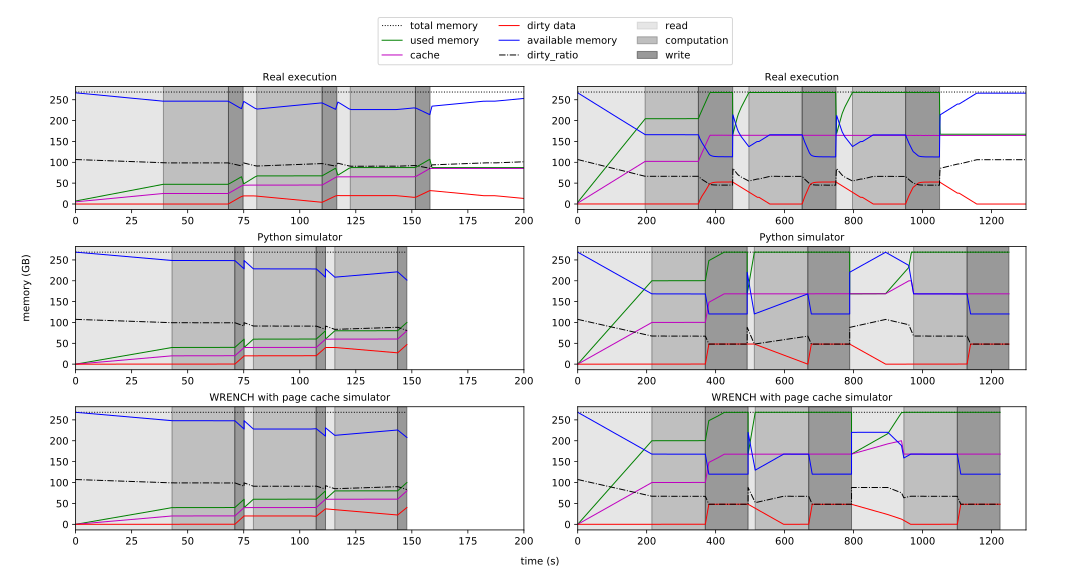
\includegraphics[width=\linewidth]{result/single/figures/single_memprof.pdf}
            \end{subfigure}
            \caption{Memory profiling results with different input file sizes \tristan{put the simulation/real conditions on the side, make them larger and use the same color code as below (pink for real, etc). Put the memory values on top, similar to how they are in the graphs below. }}
            \label{fig:single_memprof}    
            \begin{subfigure}{\linewidth}
                \centering
                   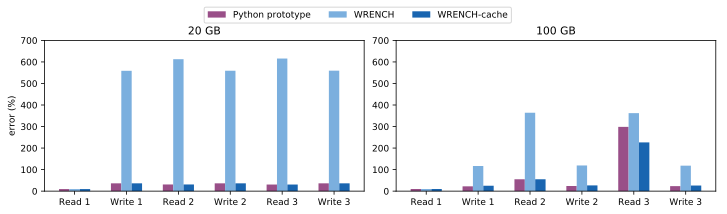
\includegraphics[width=\linewidth]{result/single/figures/single_errors.pdf}
            \end{subfigure}
            \caption{Simulation errors with different input file sizes}
            \label{fig:single_error}    
            \begin{subfigure}{\linewidth}
                \centering
                   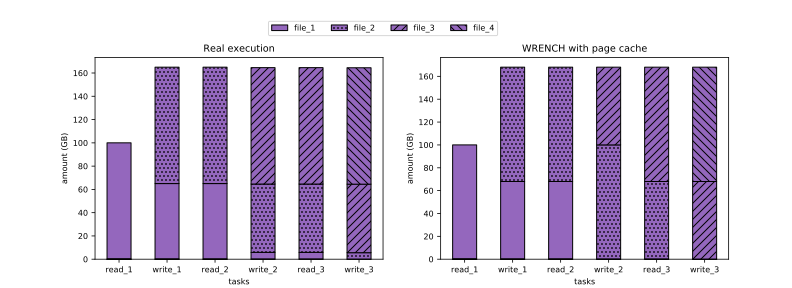
\includegraphics[width=\linewidth]{result/single/figures/cached_files.pdf}
            \end{subfigure}    
            \label{fig:single_cache}
               \caption{Amount of file data in cache after each I/O activity with 100GB of input \tristan{Make a grouped histogram (1 histogram with two bars, one for real, one for simulation). Add a grouped histogram for 20GB. Use the same color code everywhere: real should be pink.}}
            \end{figure*}            

            This longer read can be explained with the amount of cached data of files 
            at the beginning of the read in reality and simulators shown in 
            Figure~\ref{fig:single_cache}.             
            In this figure, \textit{file $<$i$>$} is the input of \textit{Read $<$i$>$} and 
            output of \textit{Write $<$i-1$>$}. 
            In the real execution, after \textit{Write 2}, which writes \textit{file 3}, 
            all data of \textit{file 3} is in cache. 
            Thus, in \textit{Read 3}, \textit{file 3} is read with memory bandwidth. 
            But in our simulator, after \textit{Write 2}, only a part of \textit{file 3} 
            remains in cache. 
            The reason is while \textit{file 3}  is being written, the page cache is saturated, 
            eviction is then evoked to evict data from page cache, make space 
            available for \textit{file 3}. 
            However, because the evicted amount is less than required, 
            some \textit{file 3} data is evicted after being written, make \textit{file 3} 
            partially cached. 
            As a result, in \textit{Read 3}, only a part of \textit{file 3} is read from cache 
            with memory bandwidth, a part of it is read from disk with disk read bandwidth, 
            which is many times slower, leading to longer read time.             
            
            In summary, in this single-threaded experiment, our model can accurately 
            simulate I/O time as well as the internal memory behavior. 
            This can help confirm that our model is on a right track and 
            it can be further improved to achieve higher accuracy.
            
        \subsection{Multi-threaded experiment}
        
            \begin{figure*}        
            \begin{subfigure}{\linewidth}
                \centering
                   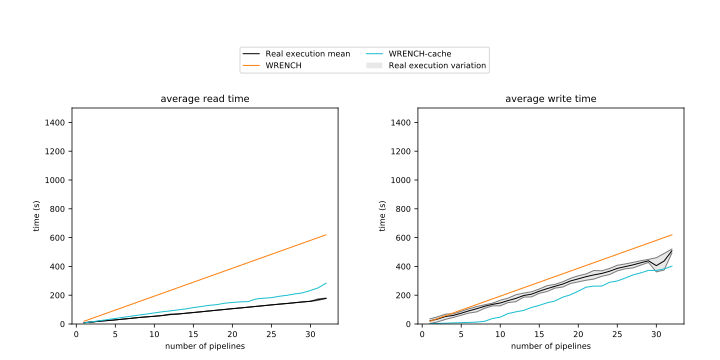
\includegraphics[width=\linewidth]{result/multi/figures/multi_local.pdf}
            \end{subfigure}        
            \caption{I/O time of concurrent pipelines with local storage. \tristan{revise caption for real execution variability: "real execution" doesnt tell what the gray shade is.}}
            \label{fig:multi_local}
            \end{figure*}        
            
            In this experiment, the results are analyzed in terms of average I/O time 
            of concurrent pipelines shown in Figure~\ref{fig:multi_local}.
            
            As is shown in the figure, when the number of pipelines increases, 
            the average read time raises accordingly because the amount of data 
            increases but memory and disk bandwidths are fixed and shared between pipelines. 
            In comparison with original WRENCH, the results from WRENCH-Ext are closer 
            to reality. 
            Especially, when it comes to the average write time, 
            although the trend in reality is more complex, our WRENCH-Ext 
            simulator can still capture the pattern in real execution.
            In both, the average write time gradually increases before surging with the 
            same slopes after the number of pipelines reaches 10. 
            This can be explained that with less than 10 concurrent pipelines, 
            the page cache is not saturated, so all files can be written entirely to 
            cache with memory bandwidth in a short time. 
            After the page cache is saturated with dirty data (at around 
            10 concurrent pipelines in this experiment), this dirty data needs 
            to be flushed in order to make space available for writing new data to cache. 
            This dirty data is flushed to disk with disk bandwidth, which is much  
            slower than memory bandwidth. 
            The more pipelines we have, the more data needs to be written, the more data 
            needs to be flushed, leading to a sharper increase in the average write time. 
            
            To conclude, the results from WRENCH-Ext simulator show that 
            our model can also simulate I/O with page cache accurately in a 
            multi-threaded application.  
            
        \subsection{Remote storage}
        
            \begin{figure*}        
            \begin{subfigure}{\linewidth}
                \centering
                   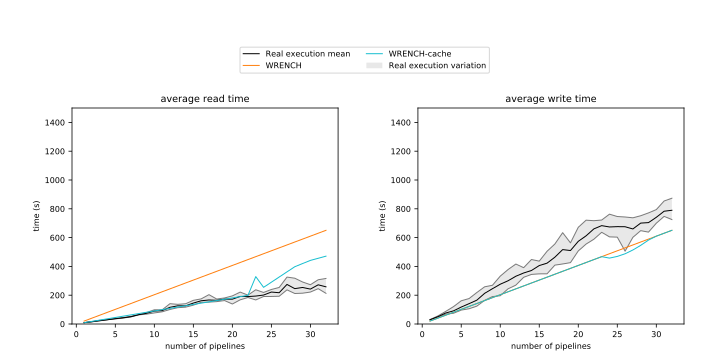
\includegraphics[width=\linewidth]{result/multi/figures/multi_nfs.pdf}
            \end{subfigure}        
            \caption{I/O time of concurrent pipelines with NFS}
            \label{fig:multi_nfs}
            \end{figure*}
        
            Similarly, the results with from the experiment with NFS are described 
            by the average I/O time shown in Figure~\ref{fig:multi_nfs}.
            In general, the average I/O time reflect a very similar level of accuracy 
            to the previous experiment results when the I/O time of pipelines 
            is very close to the real execution. 
            The simulated read time if a bit off when the number of pipelines 
            surpasses 22, with 264 GB of data in total. 
            This is due to the impact of simulated cache eviction when 
            the page cache is saturated, which has been seen in 
            Figure~\ref{fig:single_error} with 100 GB of input. 
            When it comes to write time, original WRENCH and WRENCH-Ext 
            results are identical when both are writing directly to disk.
        
        \subsection{Real application}

    \section{Discussion and Future Work}
    \label{discussion}            
            In computing infrastructures, especially those use for data-intensive applications, 
            page cache undoubtedly has certain impacts on performance. 
            Conducting simulation experiments is an effective approach to predict, 
            evaluate the performance of not only application, scheduler but also 
            infrastructure settings. 
            Unfortunately, page cache is missing in many simulation tools for HPC systems. 
            In this study, we proposed a simulation model of I/O with page cache, 
            implement it with SimGrid using WRENCH, and evaluate the results 
            with different experiments. 
            The results shows our achievements in terms of simulation accuracy 
            and the application potential in practice \tristan{what do you conclude? can we use your simulator to study big data applications on hpc clusters? under what conditions?}. 
            On the other hands, the model exposed some limitations that can be 
            further improved.
            
            Our short term future work will be re-evaluate the model with asymmetrical 
            disk bandwidths that will be released in the next SimGrid version.
            The next step is to study the detail in cache eviction mechanism to make 
            the our simulation results closer to reality. 
            Another point that needs to be further improved is the ability to configure  
            different anonymous memory usage levels of applications since it affects  
            the amount of cache used.
            We also plan to support random I/O and file readahead, as well as 
            saving and restoring disk state when hosts are turned on/off.     

\bibliographystyle{plain}
\bibliography{citation}

\end{document}
